\documentclass[letterpaper]{article}
\usepackage[ascii]{inputenc}
\usepackage[noenc]{tipa}
\usepackage{tipx}
\usepackage[geometry,weather,misc,clock]{ifsym}
\usepackage{pifont}
\usepackage{eurosym}
\usepackage{amsmath}
\usepackage{wasysym}
\usepackage{amssymb,amsfonts,textcomp}
\usepackage[T3,T1]{fontenc}
\usepackage[english]{babel}
\usepackage{color}
\usepackage{multicol}
\usepackage{array}
\usepackage{hhline}
\usepackage{hyperref}
\usepackage{graphicx}
\graphicspath{ {./images/} }
\hypersetup{colorlinks=true, linkcolor=blue, citecolor=blue, filecolor=blue, urlcolor=blue}
% Page layout (geometry)
\setlength\voffset{-1in}
\setlength\hoffset{-1in}
\setlength\topmargin{1.27cm}
\setlength\oddsidemargin{2.54cm}
\setlength\textheight{21.690998cm}
\setlength\textwidth{16.509998cm}
\setlength\footskip{0.0cm}
\setlength\headheight{1.27cm}
\setlength\headsep{1.169cm}
% Footnote rule
\setlength{\skip\footins}{0.119cm}
\renewcommand\footnoterule{\vspace*{-0.018cm}\setlength\leftskip{0pt}\setlength\rightskip{0pt plus 1fil}\noindent\textcolor{black}{\rule{0.25\columnwidth}{0.018cm}}\vspace*{0.101cm}}
% Pages styles
\makeatletter
\newcommand\ps@Standard{
  \renewcommand\@oddhead{}
  \renewcommand\@evenhead{\@oddhead}
  \renewcommand\@oddfoot{}
  \renewcommand\@evenfoot{}
  \renewcommand\thepage{\arabic{page}}
}
\makeatother
\pagestyle{Standard}
% List styles
\newcounter{saveenum}
\newcommand\liststyleWWNumiii{%
\renewcommand\theenumi{\Roman{enumi}}
\renewcommand\theenumii{\Alph{enumii}}
\renewcommand\theenumiii{\arabic{enumiii}}
\renewcommand\theenumiv{\alph{enumiv}}
\renewcommand\labelenumi{\theenumi.}
\renewcommand\labelenumii{\theenumii.}
\renewcommand\labelenumiii{\theenumiii.}
\renewcommand\labelenumiv{\theenumiv)}
}
\newcommand\liststyleWWNumi{%
\renewcommand\theenumi{\arabic{enumi}}
\renewcommand\theenumii{\alph{enumii}}
\renewcommand\theenumiii{\roman{enumiii}}
\renewcommand\theenumiv{\arabic{enumiv}}
\renewcommand\labelenumi{\theenumi.}
\renewcommand\labelenumii{\theenumii.}
\renewcommand\labelenumiii{\theenumiii.}
\renewcommand\labelenumiv{\theenumiv.}
}
\newcommand\liststyleWWNumiv{%
\renewcommand\theenumi{\arabic{enumi}}
\renewcommand\theenumii{\alph{enumii}}
\renewcommand\theenumiii{\roman{enumiii}}
\renewcommand\theenumiv{\arabic{enumiv}}
\renewcommand\labelenumi{\theenumi.}
\renewcommand\labelenumii{\theenumii.}
\renewcommand\labelenumiii{\theenumiii.}
\renewcommand\labelenumiv{\theenumiv.}
}
\newcommand\liststyleWWNumii{%
\renewcommand\labelitemi{\ding{108}}
\renewcommand\labelitemii{{\BigCircle}}
\renewcommand\labelitemiii{\ding{110}}
\renewcommand\labelitemiv{\ding{108}}
}
\newcommand\liststyleWWNumv{%
\renewcommand\labelitemi{\ding{108}}
\renewcommand\labelitemii{{\BigCircle}}
\renewcommand\labelitemiii{\ding{110}}
\renewcommand\labelitemiv{\ding{108}}
}
\title{}
\author{}
\date{2021-04-04}
\begin{document}
\clearpage\setcounter{page}{1}\pagestyle{Standard}
{\centering
\textbf{Design and Analysis of Algorithms \ }
\par}

{\centering
\textbf{DAA432C \ Assignment 06 \ }
\par}

{\centering\bfseries
Group - 14
\par}


\bigskip

{\bfseries
Kishan Tripathi \ \ \ \ \ \ \ \ \ \ \ \ \ \ \ \ \ Mukul Mohmare \ \ \ \ \ \ \ \ \ \ Anshuman Bharadwaj}

\textbf{\ \ \ \ IIT2019225 \ \ \ \ \ \ \ \ \ \ \ \ \ \ \ \ \ \ \ \ \ \ \ \ \ \ IIT2019226
\ \ \ \ \ \ \ \ \ \ \ \ \ \ \ \ \ \ \ \ \ \ \ IIT2019227}


\bigskip


\begin{multicols}{2}
{\mdseries
Abstract :}

{\bfseries\itshape
Illustrate the performance of the 0/1 Knapsack Problem and propose a parallel algorithm for the same. }

\liststyleWWNumiii
\begin{enumerate}
\item Introduction :
\end{enumerate}
The Knapsack problem is a combinatorial optimization problem where one has to maximize the benefit of objects in a
knapsack without exceeding its capacity. Given a set of items we have to find optimal packing of a knapsack. Each item
is characterized by weight and value and knapsack is characterized by capacity. Optimal packing is the one in which
weight is less or equal to the capacity and in which value is maximal among other feasible packings. 

More formally: 

Given a number of items n, their weights W = w1{\dots}{\dots}wn, their values V = v1{\dots}{\dots}vn and knapsack
capacity c, find vector X = x1{\dots}..xn so that (x1*w1 + {\dots}..xn*wn) {\textless}=c and (x1*w1 + {\dots}..xn*wn)
is maximal. [1] 


\bigskip

\liststyleWWNumiii
\setcounter{saveenum}{\value{enumi}}
\begin{enumerate}
\setcounter{enumi}{\value{saveenum}}
\item Algorithm Design :
\end{enumerate}

\bigskip

For each item we are given its weight and its value. We want to maximise the total value of all the items that we are
going to put into the knapsack such that the total weight of items is less than or equal to the knapsack's capacity.

To consider all subsets of items, there can be two cases for every item: 

\liststyleWWNumi
\begin{enumerate}
\item The item is included in the optimal subset,
\item Not included in the optimal set
\end{enumerate}

\bigskip

Therefore, the maximum value that can be obtained from n items is the max of following two values.

\liststyleWWNumiv
\begin{enumerate}
\item \ Maximum value obtained by n-1 items and W weight (excluding nth item). 
\item value of nth item plus maximum value obtained by n-1 items and W minus weight of the nth item (including nth
item).
\end{enumerate}
If the weight of the nth item is greater than W, then the nth item cannot be included and case 1 is the only
possibility. 


\bigskip

{\bfseries
Recurrence Relation : }

maximum capacity of Knapsack 

if (n=0 or W=0) 

\textbf{return} 0 


\bigskip

if (weight[n] {\textgreater} W) 

\textbf{return} \textbf{solve}(n-1, W) 

otherwise 

\textbf{return max}\{ \textbf{solve}(n-1, W), 

\textbf{solve}(n-1, W-weight[n]) \ 


\bigskip

\bigskip
{\mdseries
III. \ \ \ Code and Illustration :}


\bigskip

If we build the recursion tree for the above relation, we can clearly see that the property of overlapping subproblems
is satisfied. So, we will try to solve it using dynamic programming.


\bigskip

\ Let us define the dp solution with states i and j as 

dp[i,j]---{\textgreater} max value that can be obtained with objects u 

pto index i and knapsack capacity of j. 


\bigskip
{\bfseries
Code (Top Down Approach) :}

\textbf{\textit{\textcolor[rgb]{0.2509804,0.25882354,0.30588236}{function}}}\textcolor[rgb]{0.2509804,0.25882354,0.30588236}{
}\textbf{\textcolor[rgb]{0.2509804,0.25882354,0.30588236}{main}}\textcolor[rgb]{0.2509804,0.25882354,0.30588236}{()}

{\color[rgb]{0.2509804,0.25882354,0.30588236}
\ \ \ \ val[] = \{ 60, 100, 120 \};}

{\color[rgb]{0.2509804,0.25882354,0.30588236}
\ \ \ \ wt[] = \{ 10, 20, 30 \};}

{\color[rgb]{0.2509804,0.25882354,0.30588236}
\ \ \ \ W = 50;}

{\color[rgb]{0.2509804,0.25882354,0.30588236}
\ \ \ \ n = sizeof(val) / sizeof(val[0]);}

{\color[rgb]{0.2509804,0.25882354,0.30588236}
\ \ \ \ print knapSack(W, wt, val, n);}

\textcolor[rgb]{0.2509804,0.25882354,0.30588236}{\ \ \ \ }\textbf{\textcolor[rgb]{0.2509804,0.25882354,0.30588236}{return}}\textcolor[rgb]{0.2509804,0.25882354,0.30588236}{
0;}


\bigskip

\textbf{\textit{\textcolor[rgb]{0.2509804,0.25882354,0.30588236}{function}}}\textcolor[rgb]{0.2509804,0.25882354,0.30588236}{
}\textbf{\textcolor[rgb]{0.2509804,0.25882354,0.30588236}{knapSackRec}}\textcolor[rgb]{0.2509804,0.25882354,0.30588236}{(int
W, int wt[],int val[], int i,int** dp)}

{\color[rgb]{0.2509804,0.25882354,0.30588236}
\ \ \ \ if (i {\textless} 0)}

{\color[rgb]{0.2509804,0.25882354,0.30588236}
\ \ \ \ then}

\textcolor[rgb]{0.2509804,0.25882354,0.30588236}{\ \ \ \ \ \ \ \ }\textbf{\textcolor[rgb]{0.2509804,0.25882354,0.30588236}{return}}\textcolor[rgb]{0.2509804,0.25882354,0.30588236}{
0;}

{\color[rgb]{0.2509804,0.25882354,0.30588236}
\ \ \ \ if (dp[i][W] != -1)}

{\color[rgb]{0.2509804,0.25882354,0.30588236}
\ \ \ \ then}

\textcolor[rgb]{0.2509804,0.25882354,0.30588236}{\ \ \ \ \ \ \ \ }\textbf{\textcolor[rgb]{0.2509804,0.25882354,0.30588236}{return}}\textcolor[rgb]{0.2509804,0.25882354,0.30588236}{
dp[i][W];}

{\color[rgb]{0.2509804,0.25882354,0.30588236}
\ \ \ \ if (wt[i] {\textgreater} W) }

{\color[rgb]{0.2509804,0.25882354,0.30588236}
\ \ \ \ then}

\textcolor[rgb]{0.2509804,0.25882354,0.30588236}{\ \ \ \ \ \ \ \ dp[i][W] =
}\textbf{\textcolor[rgb]{0.2509804,0.25882354,0.30588236}{knapSackRec}}\textcolor[rgb]{0.2509804,0.25882354,0.30588236}{(W,
wt,val, i - 1,dp);}

\textcolor[rgb]{0.2509804,0.25882354,0.30588236}{\ \ \ \ \ \ \ \ }\textbf{\textcolor[rgb]{0.2509804,0.25882354,0.30588236}{return}}\textcolor[rgb]{0.2509804,0.25882354,0.30588236}{
dp[i][W];}

{\color[rgb]{0.2509804,0.25882354,0.30588236}
\ \ \ \ else}

\textcolor[rgb]{0.2509804,0.25882354,0.30588236}{\ \ \ \ \ \ \ \ dp[i][W] =
max(val[i]+}\textbf{\textcolor[rgb]{0.2509804,0.25882354,0.30588236}{
knapSackRec}}\textcolor[rgb]{0.2509804,0.25882354,0.30588236}{(W - wt[i],}

{\color[rgb]{0.2509804,0.25882354,0.30588236}
\ \ \ \ \ \ \ \ \ \ \ \ \ \ \ \ \ \ \ wt, val,i - 1, dp),}

\textcolor[rgb]{0.2509804,0.25882354,0.30588236}{\ \ \ \ \ \ \ \ \ \ \ \ \ \ \ \ \ \ \ }\textbf{\textcolor[rgb]{0.2509804,0.25882354,0.30588236}{knapSackRec}}\textcolor[rgb]{0.2509804,0.25882354,0.30588236}{(W,
wt, val,i - 1, dp));}

\textcolor[rgb]{0.2509804,0.25882354,0.30588236}{\ \ \ \ \ \ \ \ }\textbf{\textcolor[rgb]{0.2509804,0.25882354,0.30588236}{return}}\textcolor[rgb]{0.2509804,0.25882354,0.30588236}{
dp[i][W];}


\bigskip

\textbf{\textit{\textcolor[rgb]{0.2509804,0.25882354,0.30588236}{function}}}\textcolor[rgb]{0.2509804,0.25882354,0.30588236}{
}\textbf{\textcolor[rgb]{0.2509804,0.25882354,0.30588236}{knapSack}}\textcolor[rgb]{0.2509804,0.25882354,0.30588236}{(int
W, int wt[], int val[], int n)}

{\color[rgb]{0.2509804,0.25882354,0.30588236}
\ \ \ \ int** dp;}

{\color[rgb]{0.2509804,0.25882354,0.30588236}
\ \ \ \ dp = new int*[n];}

{\color[rgb]{0.2509804,0.25882354,0.30588236}
\ \ \ \ for ( i = 0; i {\textless} n; i++)}

{\color[rgb]{0.2509804,0.25882354,0.30588236}
\ \ \ \ \ \ \ \ dp[i] = new int[W + 1];}


\bigskip

{\color[rgb]{0.2509804,0.25882354,0.30588236}
\ \ \ \ for ( i = 0; i {\textless} n; i++)}

{\color[rgb]{0.2509804,0.25882354,0.30588236}
\ \ \ \ \ \ \ \ for ( j = 0; j {\textless} W + 1; j++)}

{\color[rgb]{0.2509804,0.25882354,0.30588236}
\ \ \ \ \ \ \ \ \ \ \ \ dp[i][j] = -1;}

\textcolor[rgb]{0.2509804,0.25882354,0.30588236}{\ \ \ \ }\textbf{\textcolor[rgb]{0.2509804,0.25882354,0.30588236}{return
knapSackRec}}\textcolor[rgb]{0.2509804,0.25882354,0.30588236}{(W, wt, val, n - 1, dp);}


\bigskip

\bigskip


\bigskip

{\bfseries\color[rgb]{0.2509804,0.25882354,0.30588236}
Complexity Analysis: }

\textbf{\textcolor[rgb]{0.2509804,0.25882354,0.30588236}{Time Complexity:
}}\textcolor[rgb]{0.2509804,0.25882354,0.30588236}{O(N*W). \newline
As redundant calculations of states are avoided.}

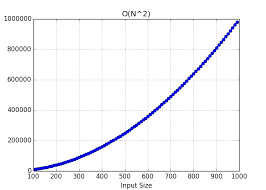
\includegraphics[scale=1.0]{complexity}
\bigskip

\textbf{\textcolor[rgb]{0.2509804,0.25882354,0.30588236}{Auxiliary Space:
}}\textcolor[rgb]{0.2509804,0.25882354,0.30588236}{O(N*W). \newline
The use of 2D array data structure for storing intermediate states}

The most optimal solution to the problem will be dp[N][W] i.e. max value that can be obtained upto index N with max
capacity of W


\bigskip

\textbf{Code (Bottom up Approach) :} 


\bigskip

\textbf{\textit{\textcolor[rgb]{0.2509804,0.25882354,0.30588236}{function}}}\textbf{\textcolor[rgb]{0.2509804,0.25882354,0.30588236}{
main}}\textcolor[rgb]{0.2509804,0.25882354,0.30588236}{()}

{\color[rgb]{0.2509804,0.25882354,0.30588236}
\ \ \ \ val[] = \{ 60, 100, 120 \};}

{\color[rgb]{0.2509804,0.25882354,0.30588236}
\ \ \ \ wt[] = \{ 10, 20, 30 \};}

{\color[rgb]{0.2509804,0.25882354,0.30588236}
\ \ \ \ W = 50;}

{\color[rgb]{0.2509804,0.25882354,0.30588236}
\ \ \ \ n = sizeof(val) / sizeof(val[0]);}

\textcolor[rgb]{0.2509804,0.25882354,0.30588236}{\ \ \ \ print
}\textbf{\textcolor[rgb]{0.2509804,0.25882354,0.30588236}{knapSack}}\textcolor[rgb]{0.2509804,0.25882354,0.30588236}{(W,
wt, val, n);}


\bigskip

\textbf{\textit{\textcolor[rgb]{0.2509804,0.25882354,0.30588236}{function}}}\textcolor[rgb]{0.2509804,0.25882354,0.30588236}{
max(int a, int b)}

\textcolor[rgb]{0.2509804,0.25882354,0.30588236}{\ \ \ \ }\textbf{\textcolor[rgb]{0.2509804,0.25882354,0.30588236}{return}}\textcolor[rgb]{0.2509804,0.25882354,0.30588236}{
(a {\textgreater} b) ? a : b;}

\textbf{\textit{\textcolor[rgb]{0.2509804,0.25882354,0.30588236}{function}}}\textcolor[rgb]{0.2509804,0.25882354,0.30588236}{
}\textbf{\textcolor[rgb]{0.2509804,0.25882354,0.30588236}{knapSack}}\textcolor[rgb]{0.2509804,0.25882354,0.30588236}{(int
W, int wt[], int val[], int n)}

{\color[rgb]{0.2509804,0.25882354,0.30588236}
\ \ \ \ i, w;}

{\color[rgb]{0.2509804,0.25882354,0.30588236}
\ \ \ \ K[n + 1][W + 1];}

{\color[rgb]{0.2509804,0.25882354,0.30588236}
\ \ \ \ for(i = 0; i {\textless}= n; i++)}

{\color[rgb]{0.2509804,0.25882354,0.30588236}
\ \ \ \ \ \ \ \ for(w = 0; w {\textless}= W; w++)}

{\color[rgb]{0.2509804,0.25882354,0.30588236}
\ \ \ \ \ \ \ \ \ \ \ \ if (i == 0 {\textbar}{\textbar} w == 0)}

{\color[rgb]{0.2509804,0.25882354,0.30588236}
\ \ \ \  then}

{\color[rgb]{0.2509804,0.25882354,0.30588236}
\ \ \ \ \ \ \ \ \ \ \ \ \ \ \ \ K[i][w] = 0;}

{\color[rgb]{0.2509804,0.25882354,0.30588236}
\ \ \ \ \ \ \ \ \ \ \ \ else if (wt[i - 1] {\textless}= w)}

{\color[rgb]{0.2509804,0.25882354,0.30588236}
\ \ \ \  then}

\textcolor[rgb]{0.2509804,0.25882354,0.30588236}{\ \ \ \ \ \ \ \ \ \ \ \ \ \ \ \ K[i][w] =
}\textbf{\textcolor[rgb]{0.2509804,0.25882354,0.30588236}{max}}\textcolor[rgb]{0.2509804,0.25882354,0.30588236}{(val[i
- 1] +K[i - 1][w - wt[i - 1]],}

{\color[rgb]{0.2509804,0.25882354,0.30588236}
\ \ \ \ \ \ \ \ \ \ \ \ \ \ \ \ \ \ \ \ \ \ \ \ \ \ \ \ \ \ \ \ K[i - 1][w]);}

{\color[rgb]{0.2509804,0.25882354,0.30588236}
\ \ \ \ \ \ \ \ \ \ \ \ else}

{\color[rgb]{0.2509804,0.25882354,0.30588236}
\ \ \ \ \ \ \ \ \ \ \ \ \ \ \ \ K[i][w] = K[i - 1][w];}

{\color[rgb]{0.2509804,0.25882354,0.30588236}
\ \ \ \ \ \ \ \ endfor}

{\color[rgb]{0.2509804,0.25882354,0.30588236}
\ \ \ \ endfor}

\textcolor[rgb]{0.2509804,0.25882354,0.30588236}{\ \ \ \ }\textbf{\textcolor[rgb]{0.2509804,0.25882354,0.30588236}{return}}\textcolor[rgb]{0.2509804,0.25882354,0.30588236}{
K[n][W];}

\bigskip
{\bfseries
Illustration :}

Let weight elements = \{1, 2, 3\}

Let weight values = \{10, 15, 40\}

Capacity=6


\bigskip

0 \ \ 1 \ \ 2 \ \ 3 \ \ 4 \ \ 5 \ \ 6


\bigskip

0 \ 0 \ \ 0 \ \ 0 \ \ 0 \ \ 0 \ \ 0 \ \ 0


\bigskip

1 \ 0 \ 10 \ 10 \ 10 \ 10 \ 10 \ 10


\bigskip

2 \ 0 \ 10 \ 15 \ 25 \ 25 \ 25 \ 25


\bigskip

3 \ 0


\bigskip

{\bfseries
Explanation:}

For filling 'weight = 2' we come 

across 'j = 3' in which 

we take maximum of 

(10, 15 + DP[1][3-2]) = 25 \ \ 

\ \ {\textbar} \ \ \ \ \ \ \ {\textbar}

{}'2' \ \ \ \ \ \ {}'2 filled'

not filled \ 


\bigskip

0 \ \ 1 \ \ 2 \ \ 3 \ \ 4 \ \ 5 \ \ 6


\bigskip

0 \ 0 \ \ 0 \ \ 0 \ \ 0 \ \ 0 \ \ 0 \ \ 0


\bigskip

1 \ 0 \ 10 \ 10 \ 10 \ 10 \ 10 \ 10


\bigskip

2 \ 0 \ 10 \ 15 \ 25 \ 25 \ 25 \ 25


\bigskip

3 \ 0 \ 10 \ 15 \ 40 \ 50 \ 55 \ 65


\bigskip

{\bfseries
Explanation:}

For filling 'weight=3', 

we come across 'j=4' in which 

we take maximum of (25, 40 + DP[2][4-3]) 

= 50


\bigskip

For filling 'weight=3' 

we come across 'j=5' in which 

we take maximum of (25, 40 + DP[2][5-3])

= 55


\bigskip

For filling 'weight=3' 

we come across 'j=6' in which 

we take maximum of (25, 40 + DP[2][6-3])

= 65

\textbf{\textcolor[rgb]{0.2509804,0.25882354,0.30588236}{Complexity
Analysis:}}\textcolor[rgb]{0.2509804,0.25882354,0.30588236}{ }

\liststyleWWNumii
\begin{itemize}
\item \textbf{\textcolor[rgb]{0.2509804,0.25882354,0.30588236}{Time
Complexity:}}\textcolor[rgb]{0.2509804,0.25882354,0.30588236}{ O(N*W). \newline
where `N' is the number of weight elements and `W' is capacity. As for every weight element we traverse through all
weight capacities 1{\textless}=w{\textless}=W}
\end{itemize}

\bigskip
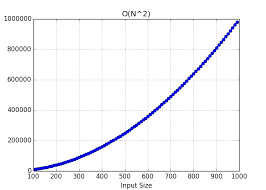
\includegraphics[scale=1.0]{complexity}

\bigskip

\liststyleWWNumii
\begin{itemize}
\item \textbf{\textcolor[rgb]{0.2509804,0.25882354,0.30588236}{Auxiliary
Space:}}\textcolor[rgb]{0.2509804,0.25882354,0.30588236}{ O(N*W). \newline
The use of 2-D array of size `N*W'.}
{\bfseries
Can we do better? }

If we observe carefully, we can see that the dp solution with states (i,j) will depend on state 

(i-1, j) or (i-1, j-wt[i-1]). In either case the solution for state (i,j) will lie in the i-lth row of the memoization
table. So at every iteration of the index, we can copy the values of the current row and use only this row for building
the solution in the next iteration and no other row will be used. Hence, at any iteration we will be using only a
single row to build the solution for the current row. Hence, we can reduce the space complexity to just O(W).


\bigskip


\bigskip


\bigskip

\textbf{Space-Optimized DP Code (for Bottom up approach) :} 


\bigskip


\bigskip

\textbf{\textit{\textcolor[rgb]{0.2509804,0.25882354,0.30588236}{function}}}\textbf{\textcolor[rgb]{0.2509804,0.25882354,0.30588236}{
main}}\textcolor[rgb]{0.2509804,0.25882354,0.30588236}{()}

{\color[rgb]{0.2509804,0.25882354,0.30588236}
\ \ \ \ val[] = \{7, 8, 4\}, wt[] = \{3, 8, 6\}, W = 10, n = 3;}

\textcolor[rgb]{0.2509804,0.25882354,0.30588236}{\ \ \ \ print
}\textbf{\textcolor[rgb]{0.2509804,0.25882354,0.30588236}{KnapSack}}\textcolor[rgb]{0.2509804,0.25882354,0.30588236}{(val,
wt, n, W) {\textless}{\textless} endl;}

{\color[rgb]{0.2509804,0.25882354,0.30588236}
\ \ \ \ return 0;}


\bigskip

\textbf{\textit{\textcolor[rgb]{0.2509804,0.25882354,0.30588236}{function}}}\textcolor[rgb]{0.2509804,0.25882354,0.30588236}{
}\textbf{\textcolor[rgb]{0.2509804,0.25882354,0.30588236}{KnapSack}}\textcolor[rgb]{0.2509804,0.25882354,0.30588236}{(int
val[], int wt[], int n, int W)}

{\color[rgb]{0.2509804,0.25882354,0.30588236}
\{}

{\color[rgb]{0.2509804,0.25882354,0.30588236}
\ \ \ \ int mat[2][W+1];}

{\color[rgb]{0.2509804,0.25882354,0.30588236}
\ \ \ \ memset(mat, 0, sizeof(mat));}


\bigskip

{\color[rgb]{0.2509804,0.25882354,0.30588236}
\ \ \ \ int i = 0;}

{\color[rgb]{0.2509804,0.25882354,0.30588236}
\ \ \ \ while (i {\textless} n) }

{\color[rgb]{0.2509804,0.25882354,0.30588236}
\ \ \ \ \ \ \ \ int j = 0; }

{\color[rgb]{0.2509804,0.25882354,0.30588236}
\ \ \ \ \ \ \ \ if (i\%2!=0)}

{\color[rgb]{0.2509804,0.25882354,0.30588236}
\ \ \ \ \ \ \ \ then}

{\color[rgb]{0.2509804,0.25882354,0.30588236}
\ \ \ \ \ \ \ \ \ \ \ \ while (++j {\textless}= W)}

{\color[rgb]{0.2509804,0.25882354,0.30588236}
\ \ \ \ \ \ \ \ \ \ \ \ \ \ \ \ if (wt[i] {\textless}= j) }

{\color[rgb]{0.2509804,0.25882354,0.30588236}
\ \ \ \ \ \ \ \ \ \ \ \ \ \ \ \ then}

\textcolor[rgb]{0.2509804,0.25882354,0.30588236}{\ \ \ \ \ \ \ \ \ \ \ \ \ \ \ \ \ \ \ \ mat[1][j]
=}\textbf{\textcolor[rgb]{0.2509804,0.25882354,0.30588236}{
max}}\textcolor[rgb]{0.2509804,0.25882354,0.30588236}{(val[i] + mat[0][j-wt[i]],}

{\color[rgb]{0.2509804,0.25882354,0.30588236}
\ \ \ \ \ \ \ \ \ \ \ \ \ \ \ \ \ \ \ \ \ \ \ \ \ \ \ \ \ \ \ \ \ \ \ \ mat[0][j] );}

{\color[rgb]{0.2509804,0.25882354,0.30588236}
\ \ \ \ \ \ \ \ \ \ \ \ \ \ \ \ else \ \ \ \ \ }

{\color[rgb]{0.2509804,0.25882354,0.30588236}
\ \ \ \ \ \ \ \ \ \ \ \ \ \ \ \ \ \ \ \ mat[1][j] = mat[0][j];}

{\color[rgb]{0.2509804,0.25882354,0.30588236}
\ \ \ \ \ \ \ \ \ \ \ \ endwhile}

{\color[rgb]{0.2509804,0.25882354,0.30588236}
\ \ \ \ \ \ \ \ \ endif}


\bigskip

{\color[rgb]{0.2509804,0.25882354,0.30588236}
\ \ \ \ \ \ \ \ else}

{\color[rgb]{0.2509804,0.25882354,0.30588236}
\ \ \ \ \ \ \ \ \ \ \ \ while(++j {\textless}= W)}

{\color[rgb]{0.2509804,0.25882354,0.30588236}
\ \ \ \ \ \ \ \ \ \ \ \ \ \ \ \ if (wt[i] {\textless}= j)}

{\color[rgb]{0.2509804,0.25882354,0.30588236}
\ \ \ \ \ \ then}

\textcolor[rgb]{0.2509804,0.25882354,0.30588236}{\ \ \ \ \ \ \ \ \ \ \ \ \ \ \ \ \ \ \ \ mat[0][j] =
}\textbf{\textcolor[rgb]{0.2509804,0.25882354,0.30588236}{max}}\textcolor[rgb]{0.2509804,0.25882354,0.30588236}{(val[i]
+ mat[1][j-wt[i]],}

{\color[rgb]{0.2509804,0.25882354,0.30588236}
\ \ \ \ \ \ \ \ \ \ \ \ \ \ \ \ \ \ \ \ \ \ \ \ \ \ \ \ \ \ \ \ \ \ \ \ \ mat[1][j]);}

{\color[rgb]{0.2509804,0.25882354,0.30588236}
\ \ \ \ \ \ \ \ \ \ \ \ \ \ \ \ else}

{\color[rgb]{0.2509804,0.25882354,0.30588236}
\ \ \ \ \ \ \ \ \ \ \ \ \ \ \ \ \ \ \ \ mat[0][j] = mat[1][j];}

{\color[rgb]{0.2509804,0.25882354,0.30588236}
\ \ \ \ \ \ \ \ i++;}


\bigskip

\textcolor[rgb]{0.2509804,0.25882354,0.30588236}{\ \ \ \ }\textbf{\textcolor[rgb]{0.2509804,0.25882354,0.30588236}{return}}\textcolor[rgb]{0.2509804,0.25882354,0.30588236}{
(n\%2 != 0)? mat[0][W] : mat[1][W];}


\bigskip
{\bfseries
Complexity Analysis:}


\bigskip

\liststyleWWNumv
\begin{itemize}
\item \textbf{Time Complexity}: O(N*W) 
\end{itemize}

\bigskip
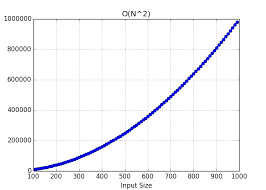
\includegraphics[scale=1.0]{complexity}

\bigskip

\liststyleWWNumv
\begin{itemize}
\item \textbf{Space Complexity}: O(N*W) 
\end{itemize}

\bigskip
{\mdseries
\ IV. \ \ \ Algorithm Analysis}

We have 3 different approaches to solve this question of 0/1 Knapsack. First one is the basic brute force approach in
which we apply recursion. Space complexity of this approach is O(n)

Where n is the number of items in the list and the time complexity of this approach is exponential i.e.,O(2\^{}n). This
solution is easy to think about but very less efficient due to its execution time.


\bigskip

Next approach is the basic optimization over the basic recursive approach . We store answers for each recursive call
each time any recursive call is called for the first time.Later we directly use the stored value rather than calling
again. 

Time complexity for this approach is O(n*m) where n is the number of items in the list and m is the capacity of the
knapsack. \ space complexity will be O(n*m) due to this 2D array for storing results for the recursive calls .


\bigskip

Last approach is bottom up approach. This algorithm's time complexity is O(n*m)

{\mdseries
\ V. \ \ \ \ Conclusion }

We can conclude that both the dynamic programming solutions are really efficient .

But now let us discuss whether this solution will work in parallel. 


\bigskip

A \textbf{parallel algorithm} is an algorithm that can execute several instructions simultaneously on different
processing devices and then combine all the individual outputs to produce the final result. We have used DP which
divides problems into subproblems but this must be noticed that subproblems are not independent . And we know that
dynamic programming can't be solved in parallel because each \textbf{subproblem} depends on the result given by other
subproblems .


\bigskip

So we reached the conclusion that a parallel algorithm is not a good idea for a 0/1 knapsack problem.


\bigskip
{\mdseries
\ VI. \ \ \ References}

\url{https://www.geeksforgeeks.org/0-1-knapsack-problem-dp-10/}

\url{https://www.geeksforgeeks.org/space-optimized-dp-solution-0-1-knapsack-problem/?ref=rp}

\url{https://www.educative.io/blog/0-1-knapsack-problem-dynamic-solution}

\url{https://www.educative.io/courses/grokking-dynamic-programming-patterns-for-coding-interviews/RM1BDv71V60}
\end{itemize}
\end{multicols}
\end{document}
